\documentclass{report}
\usepackage[utf8]{inputenc} % Required for inputting international characters
\usepackage[T1]{fontenc} % Output font encoding for international characters
\usepackage{polynom}

%%%%%%%%%%%%%%%%%%%%%%%%%%%%%%%%%
% PACKAGE IMPORTS
%%%%%%%%%%%%%%%%%%%%%%%%%%%%%%%%%
\usepackage[tmargin=2cm,rmargin=1in,lmargin=1in,margin=0.85in,bmargin=2cm,footskip=.2in]{geometry}
\usepackage{amsmath,amsfonts,amsthm,amssymb,mathtools} %general maths stuff
\usepackage[varbb]{newpxmath} %maths tools
\usepackage{xfrac} %a/b fractions
\usepackage[makeroom]{cancel}
\usepackage{mathtools}
\usepackage{bookmark}
\usepackage{enumitem}
\usepackage{hyperref,theoremref}
\hypersetup{
	pdftitle={Course Notes},
	colorlinks=true, linkcolor=black!90,
	bookmarksnumbered=true,
	bookmarksopen=true
}
\usepackage[most,many,breakable]{tcolorbox}
\usepackage{xcolor}
\usepackage{varwidth}
\usepackage{varwidth}
\usepackage{etoolbox}
\usepackage{nameref}
\usepackage{multicol,array}
\usepackage{tikz-cd}
\usepackage[ruled,vlined,linesnumbered]{algorithm2e}
\usepackage{comment} % enables the use of multi-line comments (\ifx \fi) 
\usepackage{import}
\usepackage{xifthen}
\usepackage{pdfpages}
\usepackage{transparent}
\usepackage{tikzsymbols}

\usepackage[default]{raleway}
\usepackage{sectsty}
\renewcommand*\familydefault{\sfdefault} % Force the sans-serif version of any font used
\allsectionsfont{\sffamily\mdseries\upshape} % (See the fntguide.pdf for font help)

\usepackage[nottoc,notlof,notlot]{tocbibind} % Put the bibliography in the ToC
\usepackage[titles,subfigure]{tocloft} % Alter the style of the Table of Contents
\renewcommand{\cftsecfont}{\rmfamily\mdseries\upshape}
\renewcommand{\cftsecpagefont}{\rmfamily\mdseries\upshape} % No bold!

\usepackage{calc}
\usepackage{subfig}
\usepackage{pgfplots}
\pgfplotsset{compat = newest}
\usepackage[super]{nth}
\usepackage{multicol}


%%%%%%%%%%%%%%%%%%%%%%%%%%%%%%J
% SELF MADE COLORS
%%%%%%%%%%%%%%%%%%%%%%%%%%%%%%

\definecolor{myg}{RGB}{56, 140, 70}
\definecolor{myb}{RGB}{45, 111, 177}
\definecolor{myr}{RGB}{199, 68, 64}
\definecolor{mytheorembg}{HTML}{F2F2F9}
\definecolor{mytheoremfr}{HTML}{00007B}
\definecolor{mylenmabg}{HTML}{FFFAF8}
\definecolor{mylenmafr}{HTML}{983b0f}
\definecolor{mypropbg}{HTML}{f2fbfc}
\definecolor{mypropfr}{HTML}{191971}
\definecolor{myexamplebg}{HTML}{F2FBF8}
\definecolor{myexamplefr}{HTML}{88D6D1}
\definecolor{myexampleti}{HTML}{2A7F7F}
\definecolor{mydefinitbg}{HTML}{E5E5FF}
\definecolor{mydefinitfr}{HTML}{3F3FA3}
\definecolor{notesgreen}{RGB}{0,162,0}
\definecolor{myp}{RGB}{197, 92, 212}
\definecolor{mygr}{HTML}{2C3338}
\definecolor{myred}{RGB}{127,0,0}
\definecolor{myyellow}{RGB}{169,121,69}
\definecolor{myexercisebg}{HTML}{F2FBF8}
\definecolor{myexercisefg}{HTML}{88D6D1}


%%%%%%%%%%%%%%%%%%%%%%%%%%%%
% TCOLORBOX SETUPS
%%%%%%%%%%%%%%%%%%%%%%%%%%%%
%================================
% EXAMPLE BOX
%================================

\newtcbtheorem[number within=section]{Example}{Example}
{%
	colback = myexamplebg
	,breakable
	,colframe = myexamplefr
	,coltitle = myexampleti
	,boxrule = 1pt
	,sharp corners
	,detach title
	,before upper=\tcbtitle\par\smallskip
	,fonttitle = \bfseries
	,description font = \mdseries
	,separator sign none
	,description delimiters
}
{ex}

%================================
% DEFINITION BOX
%================================
\newtcbtheorem[number within=section]{Definition}{Definition}{enhanced,
	before skip=2mm,after skip=2mm, colback=red!5,colframe=red!80!black,boxrule=0.5mm,
	attach boxed title to top left={xshift=1cm,yshift*=1mm-\tcboxedtitleheight}, varwidth boxed title*=-3cm,
	boxed title style={frame code={
			\path[fill=tcbcolback]
			([yshift=-1mm,xshift=-1mm]frame.north west)
			arc[start angle=0,end angle=180,radius=1mm]
			([yshift=-1mm,xshift=1mm]frame.north east)
			arc[start angle=180,end angle=0,radius=1mm];
			\path[left color=tcbcolback!60!black,right color=tcbcolback!60!black,
			middle color=tcbcolback!80!black]
			([xshift=-2mm]frame.north west) -- ([xshift=2mm]frame.north east)
			[rounded corners=1mm]-- ([xshift=1mm,yshift=-1mm]frame.north east)
			-- (frame.south east) -- (frame.south west)
			-- ([xshift=-1mm,yshift=-1mm]frame.north west)
			[sharp corners]-- cycle;
		},interior engine=empty,
	},
	fonttitle=\bfseries,
	title={#2},#1}{def}

%================================
% NOTE BOX
%================================


\usetikzlibrary{arrows,calc,shadows.blur}
\tcbuselibrary{skins}
\newtcolorbox{note}[1][]{%
	enhanced jigsaw,
	colback=gray!20!white,%
	colframe=gray!80!black,
	size=small,
	boxrule=1pt,
	title=\textbf{Note},
	halign title=flush center,
	coltitle=black,
	breakable,
	drop shadow=black!50!white,
	attach boxed title to top left={xshift=1cm,yshift=-\tcboxedtitleheight/2,yshifttext=-\tcboxedtitleheight/2},
	minipage boxed title=1.5cm,
	boxed title style={%
		colback=white,
		size=fbox,
		boxrule=1pt,
		boxsep=2pt,
		underlay={%
			\coordinate (dotA) at ($(interior.west) + (-0.5pt,0)$);
			\coordinate (dotB) at ($(interior.east) + (0.5pt,0)$);
			\begin{scope}
				\clip (interior.north west) rectangle ([xshift=3ex]interior.east);
				\filldraw [white, blur shadow={shadow opacity=60, shadow yshift=-.75ex}, rounded corners=2pt] (interior.north west) rectangle (interior.south east);
			\end{scope}
			\begin{scope}[gray!80!black]
				\fill (dotA) circle (2pt);
				\fill (dotB) circle (2pt);
			\end{scope}
		},
	},
	#1,
}

%================================
% Question BOX
%================================

\makeatletter
\newtcbtheorem{question}{Question}{enhanced,
	breakable,
	colback=white,
	colframe=mygr,
	attach boxed title to top left={yshift*=-\tcboxedtitleheight},
	fonttitle=\bfseries,
	title={#2},
	boxed title size=title,
	boxed title style={%
		sharp corners,
		rounded corners=northwest,
		colback=tcbcolframe,
		boxrule=0pt,
	},
	underlay boxed title={%
		\path[fill=tcbcolframe] (title.south west)--(title.south east)
		to[out=0, in=180] ([xshift=5mm]title.east)--
		(title.center-|frame.east)
		[rounded corners=\kvtcb@arc] |-
		(frame.north) -| cycle;
	},
	#1
}{def}
\makeatother


%================================
% CLAIM
%================================

\tcbuselibrary{theorems,skins,hooks}
\newtcbtheorem[number within=section]{basicproof}{Proof}
{%
	enhanced
	,breakable
	,colback = myg!10
	,frame hidden
	,boxrule = 0sp
	,borderline west = {2pt}{0pt}{myg}
	,sharp corners
	,detach title
	,before upper = \tcbtitle\par\smallskip
	,coltitle = myg!85!black
	,fonttitle = \bfseries\sffamily
	,description font = \mdseries
	,separator sign none
	,segmentation style={solid, myg!85!black}
}
{th}

%================================
% Corollery
%================================
\tcbuselibrary{theorems,skins,hooks}
\newtcbtheorem[number within=section]{Terminology}{Terminology}
{%
	enhanced
	,breakable
	,colback = myp!10
	,frame hidden
	,boxrule = 0sp
	,borderline west = {2pt}{0pt}{myp!85!black}
	,sharp corners
	,detach title
	,before upper = \tcbtitle\par\smallskip
	,coltitle = myp!85!black
	,fonttitle = \bfseries\sffamily
	,description font = \mdseries
	,separator sign none
	,segmentation style={solid, myp!85!black}
}
{th}

%%%%%%%%%%%%%%%%%%%%%%%%%%%%%%
% SELF MADE COMMANDS
%%%%%%%%%%%%%%%%%%%%%%%%%%%%%%


\newcommand{\ex}[2]{\begin{Example}{#1}{}#2\end{Example}}
\newcommand{\dfn}[2]{\begin{Definition}[colbacktitle=red!75!black]{#1}{}#2\end{Definition}}
\newcommand{\nt}[1]{\begin{note}#1\end{note}}
\newcommand{\qs}[2]{\begin{question}{#1}{}#2\end{question}}
\newcommand{\basicprf}[3]{\begin{basicproof}{#1}{#2}#3\end{basicproof}}
\newcommand{\terminology}[2]{\begin{Terminology}{#1}{}#2\end{Terminology}}

\newcommand{\plotbasic}[3][black]{ % colour func formatted
		\begin{tikzpicture}
		\begin{axis}[
				axis lines = center,
				xlabel = \(x\),
				ylabel = \(f(x)\),
			]
			
			\addplot [
				domain=-5:5, 
				samples=100, 
				color={#1},
			]
			{#2};
			\addlegendentry{#3}
		\end{axis}
	\end{tikzpicture}
}
\newenvironment{plotter}{
	\begin{tikzpicture}
		\begin{axis}[
			axis lines = center,
			xlabel = \(x\),
			ylabel = \(f(x)\),
		]
}
{
\end{axis}
\end{tikzpicture}
}


\newenvironment{unitcircled}{
\usetikzlibrary {intersections}
\begin{tikzpicture}[scale=2]
	\draw[step=.5cm,gray,very thin] (-1.2,-1.2) grid (1.2,1.2);
	\draw[->] (-1.2,0) -- (1.2,0) coordinate (x axis);
	\draw[->] (0,-1.2) -- (0,1.2) coordinate (y axis);
	\draw (0,0) circle [radius=1cm];
	
	\foreach \x/\xtext in {-1, -0.5/-\frac{1}{2}, 0, 0.5/\frac{1}{2}, 1}
	\draw (\x cm,1pt) -- (\x cm,-1pt) node[anchor=north,fill=white] {$\xtext$};
	\foreach \y/\ytext in {-1, -0.5/-\frac{1}{2}, 0.5/\frac{1}{2}, 1}
	\draw (1pt,\y cm) -- (-1pt,\y cm) node[anchor=east,fill=white] {$\ytext$};
} {
\end{tikzpicture}
}

\newcommand*\circled[1]{\tikz[baseline=(char.base)]{
	\node[shape=circle,draw,inner sep=1pt] (char) {#1};}}
\newcommand\getcurrentref[1]{%
\ifnumequal{\value{#1}}{0}
{??}
{\the\value{#1}}%
}
\newcommand{\getCurrentSectionNumber}{\getcurrentref{section}}


\newcounter{mylabelcounter}

\makeatletter
\newcommand{\setword}[2]{%
\phantomsection
#1\def\@currentlabel{\unexpanded{#1}}\label{#2}%
}
\makeatother

\tikzset{
symbol/.style={
	draw=none,
	every to/.append style={
		edge node={node [sloped, allow upside down, auto=false]{$#1$}}}
}
}
%Symbols
\newcommand{\dg}{^\circ}
\newcommand{\dang}{\measuredangle} %% Directed angle
\newcommand{\lm}{\lambda}
\newcommand{\uin}{\mathbin{\rotatebox[origin=c]{90}{$\in$}}}
\newcommand{\usubset}{\mathbin{\rotatebox[origin=c]{90}{$\subset$}}}

%Shortcuts
\newcommand{\ii}{\item}
\newcommand{\lthen}{\rightarrow}
\newcommand{\opname}{\operatorname}

%Diff/Int
\newcommand{\differen}[1][y]{\frac{\Delta #1}{\Delta x}}
\newcommand{\differend}[1][y]{\dfrac{\Delta #1}{\Delta x}}
\newcommand{\twodifferen}[1][y]{\frac{\Delta^2 #1}{\Delta x^2}}
\newcommand{\twodifferend}[1][y]{\dfrac{\Delta^2 #1}{\Delta x^2}}
\newcommand{\limit}[2]{\lim\limits_{#1 \to #2}}
\newcommand{\integratestart}[4][x]{\int_{#3}^{#4} \left( {#2} \right) d{#1}} %x/t/etc func lowerlim upperlim
\newcommand{\integrateinner}[3]{\left[ {#1} \right]_{#2}^{#3}} % func lowerlim upperlim
\newcommand{\func}[2][x]{ {#2} \left( {#1} \right)  }

\DeclareMathOperator{\cosec}{cosec}
\DeclareMathOperator{\ud}{\textit{undefined}}
\DeclareMathOperator{\rem}{rem}


%---------------------------------------
% BlackBoard Math Fonts :-
%---------------------------------------

%Captital Letters
\newcommand{\bbA}{\mathbb{A}}	\newcommand{\bbB}{\mathbb{B}}
\newcommand{\bbC}{\mathbb{C}}	\newcommand{\bbD}{\mathbb{D}}
\newcommand{\bbE}{\mathbb{E}}	\newcommand{\bbF}{\mathbb{F}}
\newcommand{\bbG}{\mathbb{G}}	\newcommand{\bbH}{\mathbb{H}}
\newcommand{\bbI}{\mathbb{I}}	\newcommand{\bbJ}{\mathbb{J}}
\newcommand{\bbK}{\mathbb{K}}	\newcommand{\bbL}{\mathbb{L}}
\newcommand{\bbM}{\mathbb{M}}	\newcommand{\bbN}{\mathbb{N}}
\newcommand{\bbO}{\mathbb{O}}	\newcommand{\bbP}{\mathbb{P}}
\newcommand{\bbQ}{\mathbb{Q}}	\newcommand{\bbR}{\mathbb{R}}
\newcommand{\bbS}{\mathbb{S}}	\newcommand{\bbT}{\mathbb{T}}
\newcommand{\bbU}{\mathbb{U}}	\newcommand{\bbV}{\mathbb{V}}
\newcommand{\bbW}{\mathbb{W}}	\newcommand{\bbX}{\mathbb{X}}
\newcommand{\bbY}{\mathbb{Y}}	\newcommand{\bbZ}{\mathbb{Z}}

%---------------------------------------
% MathCal Fonts :-
%---------------------------------------

%Captital Letters
\newcommand{\mcA}{\mathcal{A}}	\newcommand{\mcB}{\mathcal{B}}
\newcommand{\mcC}{\mathcal{C}}	\newcommand{\mcD}{\mathcal{D}}
\newcommand{\mcE}{\mathcal{E}}	\newcommand{\mcF}{\mathcal{F}}
\newcommand{\mcG}{\mathcal{G}}	\newcommand{\mcH}{\mathcal{H}}
\newcommand{\mcI}{\mathcal{I}}	\newcommand{\mcJ}{\mathcal{J}}
\newcommand{\mcK}{\mathcal{K}}	\newcommand{\mcL}{\mathcal{L}}
\newcommand{\mcM}{\mathcal{M}}	\newcommand{\mcN}{\mathcal{N}}
\newcommand{\mcO}{\mathcal{O}}	\newcommand{\mcP}{\mathcal{P}}
\newcommand{\mcQ}{\mathcal{Q}}	\newcommand{\mcR}{\mathcal{R}}
\newcommand{\mcS}{\mathcal{S}}	\newcommand{\mcT}{\mathcal{T}}
\newcommand{\mcU}{\mathcal{U}}	\newcommand{\mcV}{\mathcal{V}}
\newcommand{\mcW}{\mathcal{W}}	\newcommand{\mcX}{\mathcal{X}}
\newcommand{\mcY}{\mathcal{Y}}	\newcommand{\mcZ}{\mathcal{Z}}


%---------------------------------------
% Bold Math Fonts :-
%---------------------------------------

%Captital Letters
\newcommand{\bmA}{\boldsymbol{A}}	\newcommand{\bmB}{\boldsymbol{B}}
\newcommand{\bmC}{\boldsymbol{C}}	\newcommand{\bmD}{\boldsymbol{D}}
\newcommand{\bmE}{\boldsymbol{E}}	\newcommand{\bmF}{\boldsymbol{F}}
\newcommand{\bmG}{\boldsymbol{G}}	\newcommand{\bmH}{\boldsymbol{H}}
\newcommand{\bmI}{\boldsymbol{I}}	\newcommand{\bmJ}{\boldsymbol{J}}
\newcommand{\bmK}{\boldsymbol{K}}	\newcommand{\bmL}{\boldsymbol{L}}
\newcommand{\bmM}{\boldsymbol{M}}	\newcommand{\bmN}{\boldsymbol{N}}
\newcommand{\bmO}{\boldsymbol{O}}	\newcommand{\bmP}{\boldsymbol{P}}
\newcommand{\bmQ}{\boldsymbol{Q}}	\newcommand{\bmR}{\boldsymbol{R}}
\newcommand{\bmS}{\boldsymbol{S}}	\newcommand{\bmT}{\boldsymbol{T}}
\newcommand{\bmU}{\boldsymbol{U}}	\newcommand{\bmV}{\boldsymbol{V}}
\newcommand{\bmW}{\boldsymbol{W}}	\newcommand{\bmX}{\boldsymbol{X}}
\newcommand{\bmY}{\boldsymbol{Y}}	\newcommand{\bmZ}{\boldsymbol{Z}}
%Small Letters
\newcommand{\bma}{\boldsymbol{a}}	\newcommand{\bmb}{\boldsymbol{b}}
\newcommand{\bmc}{\boldsymbol{c}}	\newcommand{\bmd}{\boldsymbol{d}}
\newcommand{\bme}{\boldsymbol{e}}	\newcommand{\bmf}{\boldsymbol{f}}
\newcommand{\bmg}{\boldsymbol{g}}	\newcommand{\bmh}{\boldsymbol{h}}
\newcommand{\bmi}{\boldsymbol{i}}	\newcommand{\bmj}{\boldsymbol{j}}
\newcommand{\bmk}{\boldsymbol{k}}	\newcommand{\bml}{\boldsymbol{l}}
\newcommand{\bmm}{\boldsymbol{m}}	\newcommand{\bmn}{\boldsymbol{n}}
\newcommand{\bmo}{\boldsymbol{o}}	\newcommand{\bmp}{\boldsymbol{p}}
\newcommand{\bmq}{\boldsymbol{q}}	\newcommand{\bmr}{\boldsymbol{r}}
\newcommand{\bms}{\boldsymbol{s}}	\newcommand{\bmt}{\boldsymbol{t}}
\newcommand{\bmu}{\boldsymbol{u}}	\newcommand{\bmv}{\boldsymbol{v}}
\newcommand{\bmw}{\boldsymbol{w}}	\newcommand{\bmx}{\boldsymbol{x}}
\newcommand{\bmy}{\boldsymbol{y}}	\newcommand{\bmz}{\boldsymbol{z}}

\title{\huge{Pure Maths Consolidation Notes}}
\author{\huge{Jack Maguire}}
\date{}

%part,chapter,(sub(sub(sub)))section
%dfn,ex,qs,plotter

\begin{document}

\maketitle

\tableofcontents
\pagebreak

\part{Book 1}

\setcounter{chapter}{2}
\chapter{Inequalities}
\section{Basics}
Very similar to solving a normal equation with one caveat - every time you multiply by -1, you need to flip the sign.


\ex{\(5 - 3x \geq 21\)}{
	\begin{align*}
		5 - 3x &\geq 21 \\
		-3x &\geq 16 \\
		3x &\leq -16 \\
		x &\leq -\frac{16}{3}
	\end{align*}
}
\ex{\(17 + x \leq 32 + 3x \leq 21 + x\)}{
	\begin{alignat*}{2}
		17 + x &\leq 32 + 3x &&\leq 21 + x \\
		17 &\leq 32 + 2x &&\leq 21 \\
		-15 &\leq 2x &&\leq -11 \\
		-\frac{15}{2} &\leq x &&\leq -\frac{11}{2}
	\end{alignat*}
}

\section{Set Notation}
Whilst we can use \(\le\) and the other signs, we can also use set notation, which makes some easier, and is especially useful for quadratics.

\begin{align*}
	x > 4 &&\to&& \left\lbrace x: x < 4 \right\rbrace  &&\equiv&& x \in (4, \inf) \\
	-15 \leq x \leq -11 &&\to&& \left\lbrace x: -15 \leq x \leq -11 \right\rbrace  &&\equiv&& x \in [-15, -11]
\end{align*}

\section{Quadratics}
The difficulty comes with quadratics which have multiple x-solutions. We need to draw a graph, and then check which way around which we should give our answer - a single set, or a union of 2.
\ex{\(2x^2 + 5x - 3 < 0\)}{
	\begin{plotter}
		\addplot [
			domain=-5:5,
			samples=100,
			color=black,
		]
		{2*x*x + 5*x - 3};
		\addlegendentry{\(2x^2 + 5x - 3\)}
	\end{plotter}

	\begin{align*}
		2x^2 + 5x - 3 &< 0 \\
		(2x - 1)(x + 3) &< 0 \\
		-3 < x < \frac{1}{2} \\
		\left\lbrace x: -3 < x < \frac{1}{2} \right\rbrace 
	\end{align*}
}

\ex{\(x^2 > 10 - 3x\)}{
	\begin{plotter}
		\addplot [
			domain=-10:10,
			samples=100,
			color=black,
		]
		{x*x};
		\addlegendentry{\(x^2\)}
		\addplot [
			domain=-10:10,
			samples=100,
			color=blue,
		]
		{10 - 3*x};
		\addlegendentry{\(10-3x\)}
	\end{plotter}

	\begin{align*}
		x^2 + 3x - 10 &> 0 \\
		(x+5)(x-2) &> 0 \\
		\left\lbrace x: x < -5 \right\rbrace &\cup \left\lbrace x: x > 2 \right\rbrace 
	\end{align*}
}

\setcounter{chapter}{4}
\chapter{Coordinate Geometry}
A line is a function which is straight, and they have operations that can be performed on them. If the function is not of first order, then they can have multiple gradients.
All lines follow \(y = mx + c\), where \(m\) is the gradient, and \(c\) is the y-intercept.

\section{Characteristics of Lines}
\subsection{Gradient}
\dfn{Gradient}{The gradient of a line represents how shallow or deep it is. }

\begin{plotter}
	\addplot [
		domain=-5:5,
		samples=100,
		color=black,
	]
	{2*x};
	\addlegendentry{\(2x\)}
	\addplot [
		domain=-5:5,
		samples=100,
		color=blue,
	]
	{5*x};
	\addlegendentry{\(5x\)}
\end{plotter}

\dfn{Perpendicular Lines}{One line is perpendicular to another if \(m_a = \frac{-1}{m_b}\), ie they meet at \(90 \dg\)}

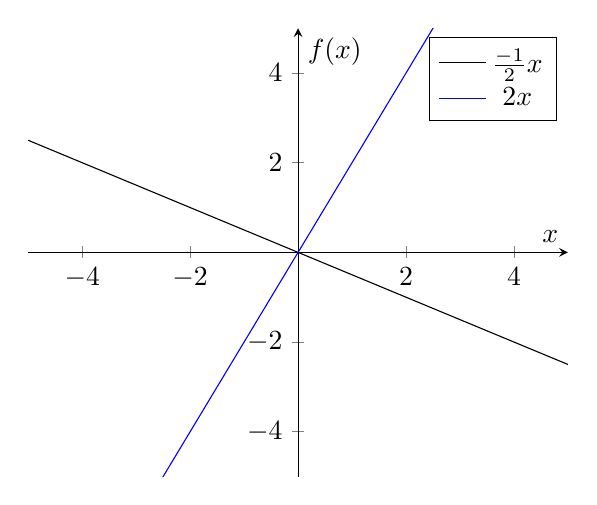
\begin{tikzpicture}
	\begin{axis}[
		axis lines = center,
		ymin=-5,ymax=5,
		xlabel = \(x\),
		ylabel = \(f(x)\),
		]
		\addplot [
		domain=-5:5,
		samples=100,
		color=black,
		]
		{-0.5*x};
		\addlegendentry{\(\frac{-1}{2}x\)}
		\addplot [
		domain=-5:5,
		samples=100,
		color=blue,
		]
		{2*x};
		\addlegendentry{\(2x\)}
	\end{axis}
\end{tikzpicture}

\subsection{Y-Intercept}

\dfn{Y Intercept}{The Y-Intercept is where the line intersects the y-axis.}
\dfn{Parallel Lines}{One line is parallel to another if the gradients are identical, but the y-intercepts are different}
\begin{plotter}
	\addplot [
		domain=-2:2,
		samples=100,
		color=black,
	]
	{x+2};
	\addlegendentry{\(x+1\)}
	\addplot [
		domain=-2:2,
		samples=100,
		color=blue,
	]
	{x-4};
	\addlegendentry{\(x-3\)}
\end{plotter}

\subsection{Lines between points}
\dfn{Midpoint}{The midpoint of a line is the average between 2 points.}
\qs{Midpoint between 2 points}{
	\ex{Between \(\left( 1,4 \right) \) and \(\left( 5,1 \right) \)}{
		\begin{align*}
			&= \left( \frac{1+5}{2} , \frac{4+1}{2} \right) \\
			&= (3, 2.5)
		\end{align*}
	}
}

\dfn{Distance}{To find the distance between 2 points, use Pythagoras.}
\qs{Distance between 2 points}{
	\ex{Between \(\left( 1,4 \right) \) and \(\left( 5,1 \right) \)}{
		\begin{align*}
			c^2 &= a^2 + b^2 \\
			c &= \sqrt{a^2 + b^2} \\
			&= \sqrt{(5-1)^2 + (4-1)^2} \\
			&= \sqrt{4^2 + 3^2}
			&= 5
		\end{align*}
	}
}

\section{Solving Line Equations}
Mainly just a question of plugging in formulas and knowing the above. One other useful thing is this:
\[ y - y_1 = m(x - x_1) \]
This equation can be used to construct a line at \((x_1, y_1)\) given gradient \(m\). This can also be used to find the y intercept.


\chapter{Circles}
Circles all follow a formula: \((x-a)^2 + (y-b)^2 = r^2\). \((a,b)\) is the centre of the circle, and \(r\) is the radius.
Questions might ask you to describe a circle given a formula - just rearrange till you can get to the formula.
When rearranging from the formula, be careful to preserve all solutions, as y is squared so you need to preserve negative values of y.

\section{Intersections between lines and circles}
Substitute into the circle equation. Make sure to check the discriminant or graph to check how many solutions exist.

\qs{Intersection between \(y=2x+1\) and \((x-3)^2 + (y+1)^2 = 64\)}{
	\begin{align*}
		(x-3)^2 + (2x+1+1)^2 &= 64 \\
		x^2 - 6x + 9 + 4x^2 + 8x + 4 &= 64 \\
		5x^2 + 2x - 51 &= 0 \\ \\
		2^2 - 4*5*-51 &> 0 \therefore \text{2 Intersections} \\ \\
		(5x+17) (x-3) &= 0 \\
		x &= 3, -3.4 \\
		y &= 2x + 1 \\
		y &= 7,-5.7 \\ \\
		&= (3,7) (-3.4, -5.8)
	\end{align*}
}

\setcounter{chapter}{7}
\chapter{Binomial Expansion}
\section{Positive Integers}

\dfn{\(\acb{n}{r} \)}{
	\[ \acb{n}{r} = \frac{n!}{r!(n-r)!} \]
	\(n\) \textit{choose} \(r\) gives the number of different ways you can choose \(r\) from a set of \(n\) things.
}
\dfn{Binomial Expansion}{
	\[ (a+b)^n = \acb{n}{0}a^nb^0 +\acb{n}{1}a^{n-1}b^1 + \acb{n}{2}a^{n-2}b^2 +\ldots + \acb{n}{n-1}a^1b^{n-1} + \acb{n}{n}a^0b^n \]
}
\ex{\(\left( 2-x^2 \right)^5\)}{
	\begin{align*}
		\left( 2-x^2 \right)^5 &= \acb{5}{0}\left( -x^2 \right)^5(2)^0 + \acb{5}{1}\left( -x^2 \right)^4(2)^1 \\ 
							   &+ \acb{5}{2}\left( -x^2 \right)^3(2)^2 + \acb{5}{3}\left( -x^2 \right)^2(2)^3 \\
							   &+ \acb{5}{4}\left( -x^2 \right)^1(2)^4 + \acb{5}{5}\left( -x^2 \right)^0(2)^5 \\
							   &= -x^{10} + (5)(2)(x^8) + (10)(4)(-x^6) + (10)(8)(x^4) + (5)(16)(-x^2) + 32 \\
							   &= -x^{10} + 10x^8 - 40x^6 + 80x^4 - 80x^2 + 32
	\end{align*}
}

\dfn{Low-Level expansions of \(\acb{n}{x}\)}{
	\begin{align*}
		\acb{n}{n} &\equiv 1 \\
		\acb{n}{1} &\equiv n \\
		\acb{n}{2} &\equiv \frac{n(n-1)}{2} \\
		\acb{n}{3} &\equiv \frac{n(n-1)(n-2)}{6}
	\end{align*}
}

\qs{Given \((3 + x)^n\), and that the coefficient of \(x^2\) is half that of \(x\), find \(n\)}{
	\begin{align*}
		x^2 \to &= \acb{n}{2}(3)^{n-2}(x)^2 \\
				&= \frac{(n)(n-1)(3)^{n-2}}{2} \\
		x   \to &= \acb{n}{1}(3)^{n-1}(x) \\
				&= n3^{n-1}
	\end{align*}
	\begin{align*}
		\frac{n(n-1)3^{n-2}}{2} &= 2n3^{n-1} \\
		n(n-1)3^{n-2} 			&= 4n3^{n-1} \\
		n(n-1) 					&= 4n*3 \\
		n^2-n					&= 12n \\
		n^2 - 13n				&= 0 \\
		n						&= 0, 13
	\end{align*}
}

\section{Binomial Estimation}
Find a formula, often given in the question, then plug in values.
\qs{Estimate \(0.975^{10}\) to 4dp}{
	\ex{Find the first 4 terms in ascending powers of x of \(\left( 1 - \frac{x}{4} \right)^{10}\)}{
		\nt{\(x^0\) is still a power of \(x\)}
		\begin{align*}
			\left( 1 - \frac{x}{4} \right)^{10} &= \acb{10}{0}(1)^10 + \acb{10}{1}(1)^9\left( -\frac{x}{4} \right) + \acb{10}{2}(1)^8\left( -\frac{x}{4} \right)^2 + \acb{10}{3}(1)^7\left( -\frac{x}{4} \right)^3 \\
			&= 1 - \frac{10}{4}x + \frac{45}{16}x^2 - \frac{120}{64}x^3 \\
			&= 1 - \frac{5}{2}x + \frac{45}{16}x^2 - \frac{15}{8}x^3
		\end{align*}	
	}
	\ex{Estimate \(0.975^{10}\) to 4dp}{
		\begin{align*}
			1 - \frac{x}{4} &= 0.975 \\
			x				&= 0.1 \\ \\
			0.975^{10} 		&\approx 1 - 0.1\frac{5}{2} + 0.1^2\frac{45}{16} - 0.1^3\frac{15}{8} \\
			&\approx 0.77625 \\
			&\approx 0.7763
		\end{align*}
	}
}

\section{Fractions}
\dfn{General Binomial Expansion}{
	\begin{align*}
		(1 + x)^n &= 1 + nx + \frac{n(n-1)}{2!}x^2 + \frac{n(n-1)(n-2)}{3!}x^3 \\
				  &+ \frac{n(n-1)\ldots(n-r+1)}{r!}x^r
	\end{align*}
	Valid for \(\left| x \right| < 1\).
}
\qs{\((1-2x)^\frac{1}{2}\), where \(\left| x \right| < \frac{1}{2}\), find ascending powers of \(x\) up to and including \(x^3\)}{
	\begin{align*}
		&= 1 + \frac{1}{2}x + \frac{\frac{1}{2}\left( \frac{1}{2} - 1 \right)}{2}x^2
	\end{align*}
}

\chapter{Trig Ratios}
\input{Maths/Pure/B1/9_TrigRatios.tex}

\chapter{Trig Functions}
\input{Maths/Pure/B1/10_TrigFunctions.tex}

\setcounter{chapter}{11}
\chapter{Differentiation}
\input{Maths/Pure/B1/12_Differentitation.tex}

\chapter{Integration}
\input{Maths/Pure/B1/13_Integration.tex}

\chapter{Logs \& Exponents}
\section{Logarithms}

\dfn{Logarithms}{
	\(a^x = y \therefore \log_ay=x\)
}
\begin{tabular}{cc}
	Exponential Fact & Logarithm Fact \\ \\
	\hline \\
	\(10^3 = 1000\) & \(\log_{10}1000 = 3\) \\ \\
	\(5^4 = 625\) & \(\log_5{625} = 4\) \\ \\
	\(36^{\frac{1}{2}} = 6\) & \(log_{36}6 = \frac{1}{2}\) \\ \\
	\(2^{-3} = \frac{1}{8}\) & \(log_2{\frac{1}{8}} = 3\)
\end{tabular}

\subsection{Log Laws}
\dfn{Log \& Index Laws}{
	\begin{tabular}{cc}
		Laws of Indices & Laws of Logs \\ \\
		\hline \\
		\(a^x * a^y = a^{x+y}\) & \(\log_ax + \log_ay = \log_amn\) \\ \\
		\(a^x \div a^y = a^{x-y}\) & \(\log_ax - \log_ay = \log_a\frac{x}{y}\) \\ \\
		\(\left( a^x \right) ^y = a^{xy}\) & \(\log_ax * \log_ay = \log_am^n\)
	\end{tabular}
}

\qs{\(\log_4\frac{x}{x-1} = \log_43 + log_42\)}{
	\begin{align*}
		\log_4\frac{x}{x-1} &= \log_46 \\
		\frac{x}{x-1} &= 6 \\
		x &= 6x - 6 \\
		\ldots
	\end{align*}
}
\qs{\(\log_74x = \log_7\frac{1}{x-6} + 1\)}{
	\begin{align*}
		\log_7\frac{4}{\frac{1}{x-6}} &= 1 \\
		\log_74x(x-6) &= 1 \\
		\log_74x^2-24x &= 1 \\
		4x^2-24x &= 7 \\
		\ldots
	\end{align*}
}
\qs{\(2^x=75\)}{
	\begin{align*}
		x &= \log_275 \\
		x &= 6.23
	\end{align*}
}
\qs{\(5^{2x} - 6\left( 5^x \right) = 0\)}{
	\begin{align*}
		\text{let } y &= 5^x \\
		y^2 - 6y - 7 &= 0 \\
		(y - 7)(y + 1) &= 0 \\
		\text{Logarithms always positive} \therefore y &= 7 \\
		5^x &= 7 \\
		x &= log_57 \\
		x &= 1.21 \\
	\end{align*}
}
\qs{\(3^{2x+1} = 2^{5x}\)}{
	\begin{align*}
		\log_e3^{2x+1} &= \log_e2^{5x} \\
		(2x+1)\log_e3 &= (5x)\log_e2 \\
		2(\log_e3)x + \log_e3 &= 5(log_e2)x \\
		\log_e3 &= 5(\log_e2)x - (2log_e3)x \\
		\log_e3 &= x(5log_e2 - 2loge_3) \\
		x &= \frac{log_e3}{5log_e2 - 2loge_3} \\
		x &= 0.866
	\end{align*}
}


\section{Exponentials}
\begin{plotter}
	\addplot [
		domain=-2:2,
		samples=100,
		color=black,
	]
	{2^x};
	\addlegendentry{\(2^x\)}
	\addplot [
		domain=-2:2,
		samples=100,
		color=black,
	]
	{2*2^x};
	\addlegendentry{\(2*2^x\)}
\end{plotter}

Graphs with anything to the power of \(x\) always have a y-intercept of 1, because anything to the power of 0 is equal to 1.


\subsection{Euler's Number - \(e\)}
\dfn{\(e\)}{
	\(e\) is defined as having the following characteristics:
	\begin{itemize}
		\ii \(y = e^x\), \(\differen = e^x\)
		\ii \(y = e^{kx}\), \(\differen = ke^{kx}\)
	\end{itemize}
}
\qs{\(y = Ae^{kx}\), and passes through \((0,6)\) and \(1,9\). Find \(A\) and \(k\)}{
	\begin{align*}
		6 &= Ae^0 \\
		A &= 6 \\ \\	
		9 &= 6e^k \\
		e^k &= \frac{9}{6} \\
		k &= \ln\frac{9}{6} \\
		k &= 0.41
	\end{align*}
}

\section{Modelling With Exponentials}
All Exponentials can be written with \(e\), which makes calculus much easier.

Given \(y = Ae^{kx}\), if \(k > 0\) we get exponential growth, and if \(k < 0\) then we get exponential decay.

% got up to just before 29/9 DJI before lunch


\part{Other Bits}
\setcounter{chapter}{0}
\chapter{Transforming \& Sketching Graphs}
\section{Graph Appearances}
\subsection{Transformations}

\dfn{Translation}{
	\begin{itemize}[]
		\ii The graph of \( f(x-a) \) is the graph of \( f(x) \) translated right by \(a\) units.
		\ii The graph of \( f(x)+b\) is the graph of \( f(x) \) translated upwards by \(b\) units.
	\end{itemize}
}
\dfn{Scaling}{
	\nt{Never say shrink: always say stretch by a factor \( e \) where \( |e| < 1 \)}
	\begin{itemize}[]
		\ii The graph of \(cf(x)\) is the graph of \(f(x)\) stretched vertically by a factor of \(c\).
		\ii The graph of \(f(dx)\) is the graph of \(f(x)\) stretched horizontally by a factor of \(d^{-1}\).
	\end{itemize}
}
\ex{Basic Graph Transformations}{
	\begin{plotter}
		\addplot [
		domain=-5:5,
		samples=100,
		color=black,
		]
		{x^2};
		\addlegendentry{\(x^2\)}
	\end{plotter}
	
	\hbox{
		\begin{plotter}
			\addplot [
			domain=-5:5,
			samples=100,
			color=red,
			]
			{(x-2)^2};
			\addlegendentry{\((x-2)^2\)}
			
			\addplot [
			domain=-5:5,
			samples=100,
			color=orange,
			]
			{(x)^2+10};
			\addlegendentry{\((x)^2+10\)}
		\end{plotter}
		
		\begin{plotter}
			\addplot [
			domain=-5:5,
			samples=100,
			color=blue,
			]
			{3*(x^2)};
			\addlegendentry{\(3(x^2)\)}
			
			\addplot [
			domain=-5:5,
			samples=100,
			color=purple,
			]
			{(x/2)^2};
			\addlegendentry{\((0.5x)^2\)}
		\end{plotter}
	}
}

\subsection{Combining Transformations}

\qs{Combining Transformations}{
	\[
	y = f(-2x)
	\]
	
	This is obtained from \(f(x)\) by doing the following:
	\begin{enumerate}
		\item Flip horizontally.
		\item Stretch horizontally by a factor of \(0.5\).
	\end{enumerate}
}
\qs{Combining Transformations}{
	\[
	y = cf(\frac{1}{a} * (x-b)) + d
	\]
	
	This is obtained from \(f(x)\) by doing the following:
	\begin{enumerate}
		\item Shift to the right \(b\) units.
		\item Stretch horizontally by a factor of \(a\).
		\item Stretch vertically by a factor of \(c\).
		\item Shift upwards by \(d\) units.
	\end{enumerate}
}


\pagebreak
\subsection{Graph Shapes}
\ex{Basic Power Graphs}{
	\hbox {
		\plotbasic[blue]{x}{\(x\)}
		\plotbasic[red]{x^2}{\(x^2\)}
	}
	\hbox {
		\plotbasic[blue]{x^3}{\(x^3\)}
		\plotbasic[red]{x^4}{\(x^4\)}
	}
	\hbox {
		\plotbasic[blue]{1/x}{\(x^{-1}\)}
		\plotbasic[red]{-1/x}{\({-x}^{-1}\)}
	}
}

These are all of the basic graph shapes, and can be transformed just like \(y = x^2\) above.

\pagebreak
\section{Solving Using Graphs}
Find one or more \(y =\ldots \) equation, plot it, find the x position of any intercepts. If only one equation, find intersections with \(y = 0\).

\qs{Solving \(5 = 6x + 8\)}{
	\begin{align}
		5  & = 6x + 8 \\
		-3 & = 6x     \\
	\end{align}
	
	\ex{Using Algebra}{
		\begin{align}
			6x & = -3           \\
			x  & = \frac{6}{-3} \\
			x  & = -\frac{1}{2}
		\end{align}
	}
	
	\ex{Using a Graph}{
		\[ y = 6x + 3  \]
		\plotbasic{6*x+3}{\(6x + 3 \)}
		Intersects at \(-\frac{1}{2}\).
	}
	
	Whilst this might seem less useful for basic equations, this can become much more useful for more complicated questions like below.
}

\qs{Finding the intersection of  \(y = 3x^2 -2x - 21\) and \(y = (x-3)(x+3)\)}{
	\ex{Using Algebra}{
		\begin{enumerate}
			\ii Set equal to each other
			\ii Simplify
			\ii Check how many roots exist using the discriminant
			\ii Work out all roots (possibly using factor theorem which can take a while)
		\end{enumerate}
		\begin{align}
			3x^2 -2x - 21  & = (x-3)(x+3) \\
			3x^2 -2x - 21  & = x^2 - 9    \\
			2x^2 -2x - 12  & = 0          \\
			x^2 - x - 6    & = 0          \\
			(x - 3)(x + 2) & = 0          \\
			x              & = 3, -2
		\end{align}
	}
	
	\ex{Using a Graph}{
		\begin{enumerate}
			\ii Plot
			\ii Check intersections.
		\end{enumerate}
		
		\begin{plotter}
			\addplot [
			domain=-7.5:7.5,
			samples=100,
			color=black,
			]
			{3*x^2 - 2*x - 21};
			\addlegendentry{\(3x^2 -2x -21\)}
			
			\addplot [
			domain=-7.5:7.5,
			samples=100,
			color=black,
			]
			{(x-3)*(x+3)};
			\addlegendentry{\((x+3)(x-3)\)}
		\end{plotter}
		
		Intersects at \(x = -2, 3\).
	}
}

\chapter{Polynomial Division, Factor Theorem \& Cubics}
\section{Polynomial Division}
Any expression \(\frac{\func{f}}{\func{g}}\) can be expressed as \( \func{g} \rem \func{r}\). For example, \(\frac{11}{4} \equiv 2 \rem 3\).

There are 2 main methods of dividing polynomials - Long Division and Synthetic. Synthetic is usually considered easier, but a question might ask for Long Division, so learn both.
\qs{\(x^3 - 17x + 6 \quad \div \quad x - 3\)}{
	\ex{Synthetic Division}{
		Synthetic Division isn't very hard, but has steps you need to carefully follow. Firstly, copy all of the coefficients into the top row, and the negative of the divisor constant into the left column in the row below. For the first coefficient, copy it directly to the bottom. Then, for all of the others follow these steps:
		\begin{enumerate}
			\ii Multiply the result from the order above by the negative of the constant, and copy it to the middle row. 
			\ii Add that to the original and place the result in the bottom row.
		\end{enumerate}
		\polyhornerscheme[x=3]{x^3 - 17x + 6}
		\[\therefore \frac{x^3 - 17x + 6}{x - 3} = x^2 + 3x - 8 \rem -18\]
	}
	\ex{Long Division}{
		Long Division involves a few main steps, which you repeat for every term of the dividend. It starts with laying out the equation in the box as you would for normal long division, and then you do the following:
		\begin{enumerate}
			\ii Divide the dividend term by the divisor term an order below, and add that to the result at the top
			\ii Copy the dividend term a row below
			\ii Multiply the next dividend term by the negative of the constant in the divisor.
			\ii Treat what you've written down as long subtraction.
			\ii Copy the rest of the row down into the results bit.
		\end{enumerate}
		Continue until you get to a lone constant, and that is the remainder
		
		\polylongdiv{x^3 + 0x^2 - 17x + 6}{x - 3}
		\[\therefore \frac{x^3 - 17x + 6}{x - 3} = x^2 + 3x - 8 \rem -18\]
	}
}

\section{Factor Theorem}
The factor theorem is a method of solving cubic equations.
\dfn{Factor Theorem}{
	Given \(\func{f}\), if \(f(y)\) is a solution, then \(\left( x-y \right)\) is a factor of \(\func{f}\)
}

To solve an equation using factor theorem, usually we need to follow a few steps:
\begin{enumerate}
	\ii Work through factors of the constant until you find one that is a factor of the whole equation.
	\ii Create a trial factorising function.
	\ii Expand the faux-factorised function, and equate coefficients.
	\ii Write a proper expanded function.
	\ii Properly factorise.
\end{enumerate}

\qs{Given one solution is an integer, solve \(2x^3 + x^2 - 18x + 9\)}{
	\ex{Solving with Factor Theorem}{
		\begin{align*}
			\func{f}  	 &= 2x^3 + x^2 - 18x - 9 \\
			\func[1]{f}  &= 2 + 1 - 18 - 9 \neq 0 \\
			\func[-1]{f} &= 2 + 1 + 18 - 9 \neq 0 \\
			\func[3]{f}  &= 2*27 + 9 - 54 - 9 = 0 \\
			\func[3]{f}  &= 0 \quad \therefore \left( x-3 \right) \text{is a factor} \\
			\\
			\func{f} &= \left( x-3 \right) \left( 2x^2 + bx + 3 \right) \\
					 &= \ldots - 6x^2 + bx^2 + \ldots \\
			b-6 	 &= 1 \\
			b		 &= 7 \\
			\\
			\func{f} &= \left( x-3 \right) \left( 2x^3+7x+3 \right) \\
					 &= \left( x-3 \right) \left( 2x+1 \right) \left( x+3 \right) \\
			\therefore x &= -3, \frac{1}{2}, 3 
		\end{align*}
	}
}


\part{Book 2}

\setcounter{chapter}{0}
\chapter{Algebraic Methods}
\input{Maths/Pure/B2/1_AlgebraicMethods.tex}

\chapter{Functions \& Graphs}
\input{Maths/Pure/B2/2_FunctionsGraphs.tex}

\chapter{Sequences \& Series}
\dfn{\(a\) and \(d\) notation} {
	\begin{tabular}{rl}
		Symbol  & Meaning \\
		\hline
		\(U_n\) & \(n\)\textsuperscript{th} term \\
		\(S_n\) & Sum of terms up to and including \(U_n\) \\
		\(a\) & First Term (AKA \(U_1\)) \\
		\(d\) & Common Difference \\
		\(r\) & Common Factor \\
	\end{tabular}
}
\dfn{Sigma Notation}{
	\[ \sum_{r=1}^{10} U_r = U_1 + U_2 + \ldots + U_{10} = S_{10} \]
}

\section{Arithmetic Series}
\subsection{\(U_n\)}
\dfn{Term Formula}{
	\[U_n = a + (n-1)d\]
}

\qs{\(U_5 = 17\), \(U_4 = 3\), Find \(U_n\)}{
	\begin{align*}
		17 &= a + 4d \\
		3 &= a + 8d \\ \\
		& \text{Solve Simultaneous Equations} \\
		a &= 31 \\
		d &= -\frac{7}{2} \\ \\
		U_n &= 31 +  \left( n-1 \right)  \left( -\frac{7}{2} \right) \\
		&= -\frac{7}{2}n + 34\frac{1}{2}
	\end{align*}
}

\subsection{\(S_n\)}
\dfn{Sum Formula}{
	\begin{align*}
		S_n &= \frac{n}{2}\left( \text{First} - \text{Last} \right) \\
		& \therefore \\
		S_n &= \frac{n}{2}\left( 2a + (n-1)d \right)
	\end{align*}
}

\qs{\( \sum_{n=1}^{20}5n-3 \)}{
	\begin{align*}
		\sum_{n=1}^{20}5n-3 &= \frac{n}{2}\left( 2a + (n-1)d \right) \\
		&= 10(4+19*5) \\
		&= 990
	\end{align*}
}


\section{Geometric Sequences}
\subsection{\(U_n\)}
\dfn{Term Formula}{\[U_n = ar^{n-1}\]}

\qs{Given terms \(3, x, x+6\), find \(U_{10}\)}{
	\begin{align*}
		\frac{x}{3} &= \frac{x+6}{x} \\
		x^2 &= 3x + 18 \\
		0 &= x^2 - 3x - 18 \\
		0 &= (x - 6)(x+3) \\
		x &= 6,-3 \\
	\end{align*}

	\begin{multicols}{2}
	\noindent
	\begin{align*}
		x &= 6 \\
		U &= 3,6,12 \\
		(a,r) &= (3,2) \\
		U_n &= 3*2^{n-1} \\
		U_{10} &= 3*2^9 \\
		&= 136
	\end{align*}
	\columnbreak
	\begin{align*}
		x &= -3 \\
		U &= 3,-3,3 \\
		(a,r) &= (3,-1) \\
		U_n &= 3*-1^{n-1} \\
		U_{10} &= 3*2^9 \\
		&= -3
	\end{align*}
	\end{multicols}

	\[\therefore x = -3, 136\]
}
\qs{Given terms \(2,6,18\), find \(n\) where \(U_n > 500,000\)}{
	\begin{align*}
		(a,r) &= (2,3) \\
		U_n &= 2 * 3^{n-1} \\
		2 * 3^{n-1} &> 500000 \\
		3^{n-1} &> 250000 \\
		n &> \log(250000)  1\\
		n &> 12.3 \\
		n &= 13 \\
	\end{align*}
}



\subsection{\(S_n\)}
\dfn{Sum Formula}{\[ S_n = \frac{a\left( 1-r^n \right) }{1-r} \]}

\qs{\(1024 - 512 + 256 - 128 + \ldots + 1 = x\), find \(x\)}{
	\begin{align*}
		(a, r) &= (1024, -\frac{1}{2}) \\
		n &=\log_2(1024) + 1 \\
		&= 11 \\
		S_n &= a\frac{1-r^n}{1-4} \\
		&= 1024 \frac{1+\frac{1}{2}^{11}}{1+\frac{1}{2}} \\
		&= 683
	\end{align*}
}

\subsection{Geometric Sequences to Infinity}
\dfn{Sum to Infinity}{
	If \(U_n = ar^n\), and \(\left| r \right|  < 1\), then \(S_\infty = \frac{a}{1-r} \).
}
\dfn{Convergent vs Divergent}{
	Given \(U_n = a + (n-1)d\)
	\begin{alignat*}{2}
	\limit{U_n}{\infty} & d > 0 & \text{Tends to } \infty\\
				   		  & d < 0 & \text{Tends to } -\infty\\
	\limit{S_n}{\infty}    & d > 0 & \text{Tends to } \infty\\
						  & d < 0 & \text{Tends to } -\infty\\
	\end{alignat*}
}


\section{Recurrence Relations}
\dfn{Recurrence Relations}{
	A recurrence relation is a term-to-term rule for a sequence denoted by \(U_{n+1} = \func[U_n]{f}\), with a value given for \(U_1\)
}

\setcounter{chapter}{5}
\chapter{Trig Functions}
\input{Maths/Pure/B2/6_TrigFunctions.tex}

\chapter{Trig Modelling}
\input{Maths/Pure/B2/7_TrigModelling.tex}

\chapter{Parametric Equations}
\input{Maths/Pure/B2/8_Parametrics.tex}

\chapter{Differentiation}
\input{Maths/Pure/B2/9_Differentiation.tex}

\setcounter{chapter}{10}
\chapter{Integration}
\input{Maths/Pure/B2/11_Integration.tex}

\end{document}
